\documentclass{article}

\usepackage[utf8]{inputenc}
\usepackage{url}
\usepackage{amsmath}
\def\UrlFont{\em}
\usepackage{indentfirst}

\title{Trabalho de Visão Relatório}
\author{Felipe Leivas Machado - 262528 \and Priscila Cavalli Rachevsky - 261573 }

\usepackage{natbib}
\usepackage{graphicx}
\usepackage{capt-of}

\begin{document}

\maketitle

\section{Introdução}
    A partir de uma imagem com linhas que representavam os eixos \(X\) e \(Y\) de um plano cartesiano e uma parábola precisava a plotar essas linhas novamente, garantindo que os eixos eram perpendiculares e garantindo que a parábola seguisse uma equação de segundo grau. Para isso, precisou seguir esses passos:
   \begin{itemize}
       \item Extrair uma imagem de bordas
       \item Identificar os eixos \(X\) e \(Y\)
       \item Remover os eixos
       \item Forçar eixos perpendiculares 
       \item Identificar a parábola
       \item Desenhar a parábola
   \end{itemize}
\section{Implementação}
   \subsection{Extrair uma imagem de bordas}
   Primeiramente, a imagem foi transformada para ter apenas tons cinza. Então, se aplicou o filtro Gaussiano com kernel tamanho 7 para diminuir eventuais ruídos. Dessa forma, aplicou-se binarização, no qual o linear tinha o valor de 143.
   \begin{figure}[h!]
   \centering
    \subfigure
        {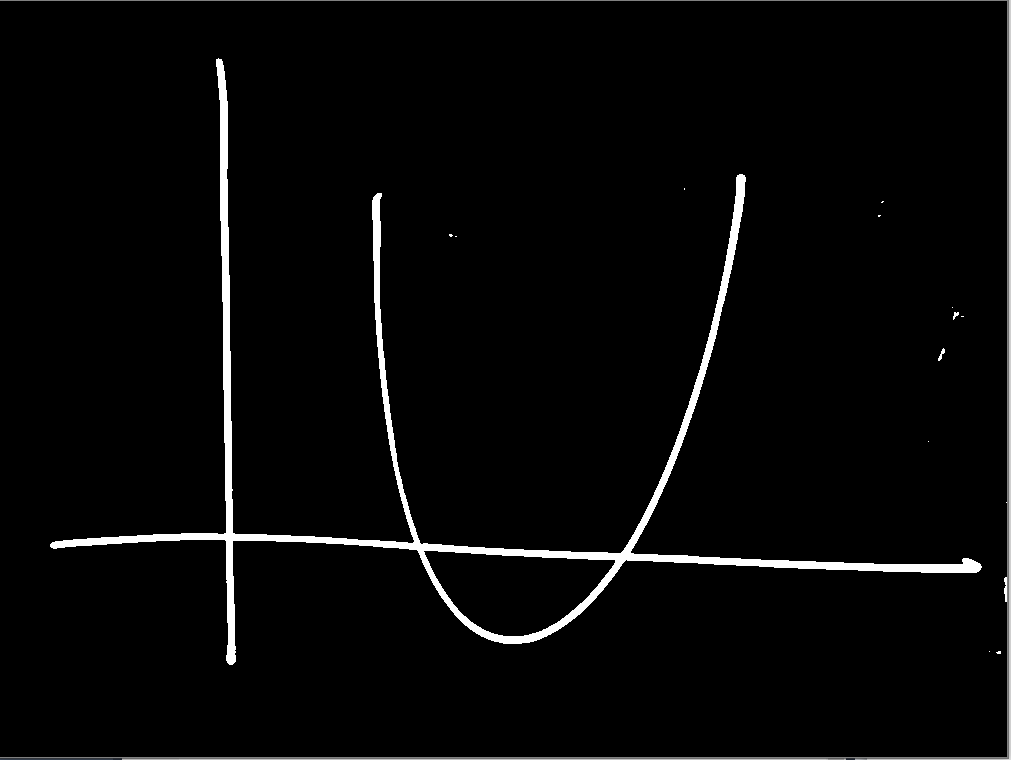
\includegraphics[scale=0.17]{exemplo1_edge.PNG}}
    \subfigure
        {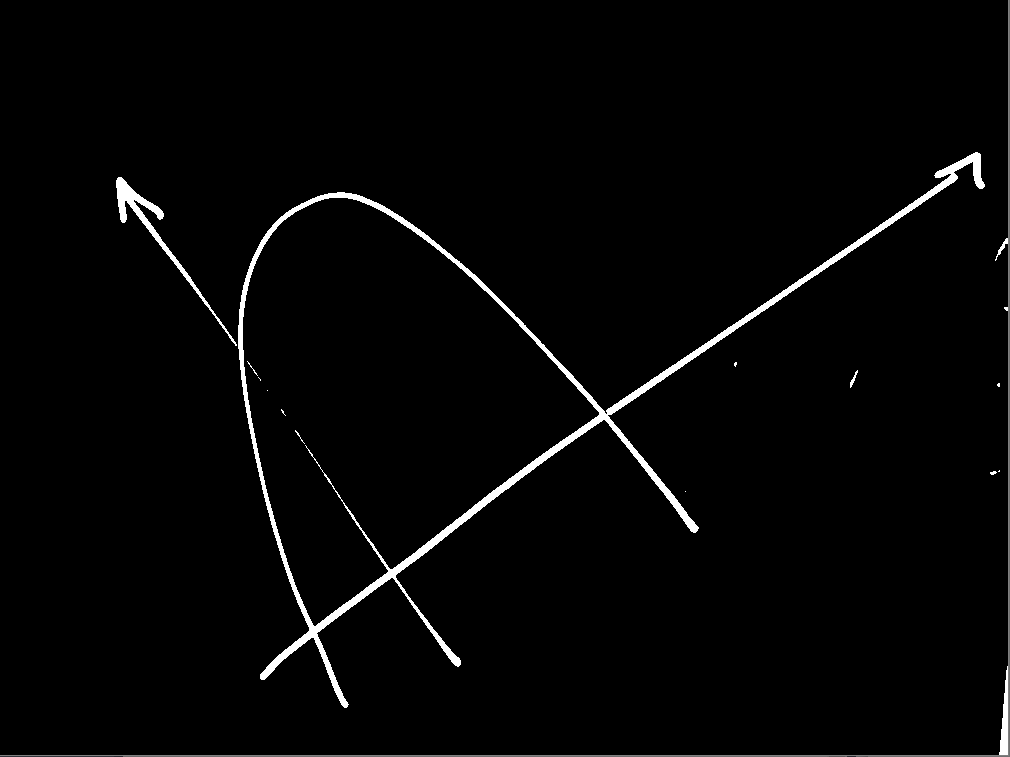
\includegraphics[scale=0.17]{exemplo2_edge.PNG}}
    \subfigure
        {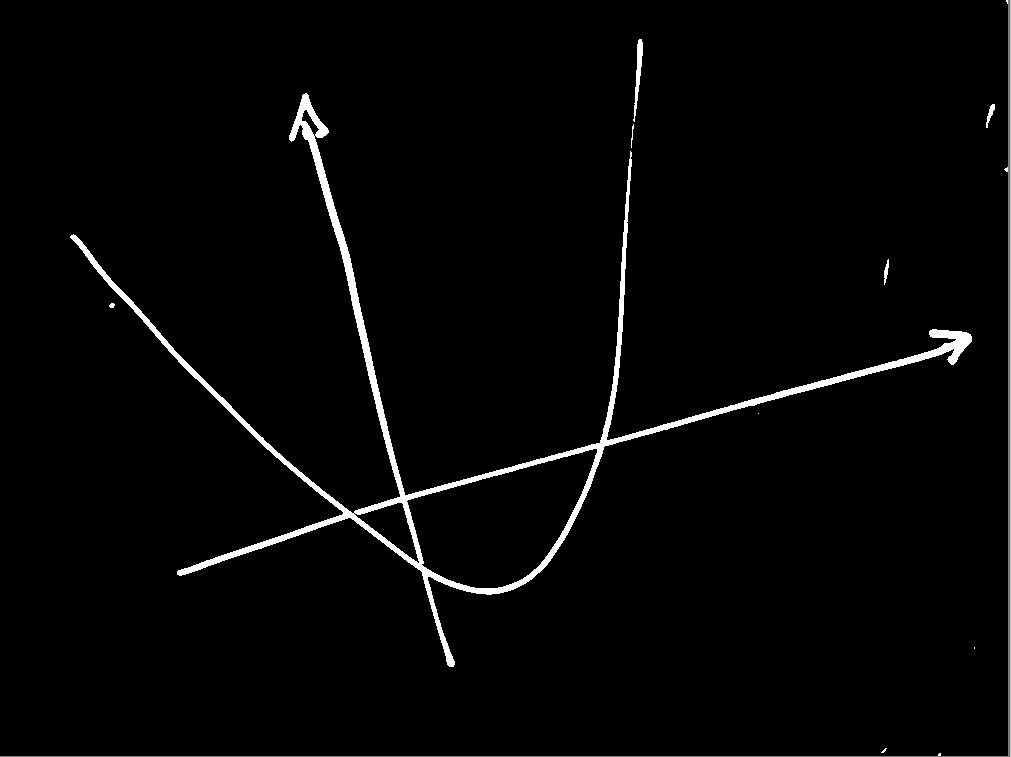
\includegraphics[scale=0.17]{exemplo3_edge.PNG}}
    \caption{Imagens de bordas}
    \end{figure}

   \subsection{Identificar os eixos \(X\) e \(Y\)}
   Usou-se Hough para identificar todas linhas que atendiam aos critérios de:
   \begin{itemize}
       \item    Tamanho mínimo de 300 pixels
       \item    Gap máximo de 50 de gap 
   \end{itemize}
   Então, identificou-se que as linhas eram eixo \(X\) quando a diferença entre seus 2 pontos era maior no \(x\) do que no \(y\), ou seja, \((x_1 - x_2)^2 > (y_1 - y_2) ^2\), caso contrário, a linha representava o eixo \(Y\).
  Foi usado minimos quadráticos para determinar a reta que passava pelos extremidades das linhas do eixo \(X\) para ser a reta do eixo \(X\) e para o eixo \(Y\) se pegou todas linhas que estavam próximas a maior linha de todas que foram classificadas do eixo \(Y\) e se utilizou minimos quadráticos para determinar a reta do eixo \(Y\), foi utilizada essa estratégia pois em alguns casos partes da parábola eram reconhecidas como sendo do eixo Y.
 
 \subsection{Forçar eixos perpendiculares}
   Com esses retas se determinou a origem do sistema. E utilizamos a reta \(X\) como base para se calcular a reta \(Y\), pegando uma reta perpendicular a \(X\) e que passase pela origem do sistema assim se teve a reta \(Y\)
   
   \subsection{Remover os eixos}
   Utilizou as retas dos eixo perpendiculares e foi removido todos os pixels que estivessem a pelo menos 80 pixels de distância
   \begin{figure}[h!]
   \centering
    \subfigure
        {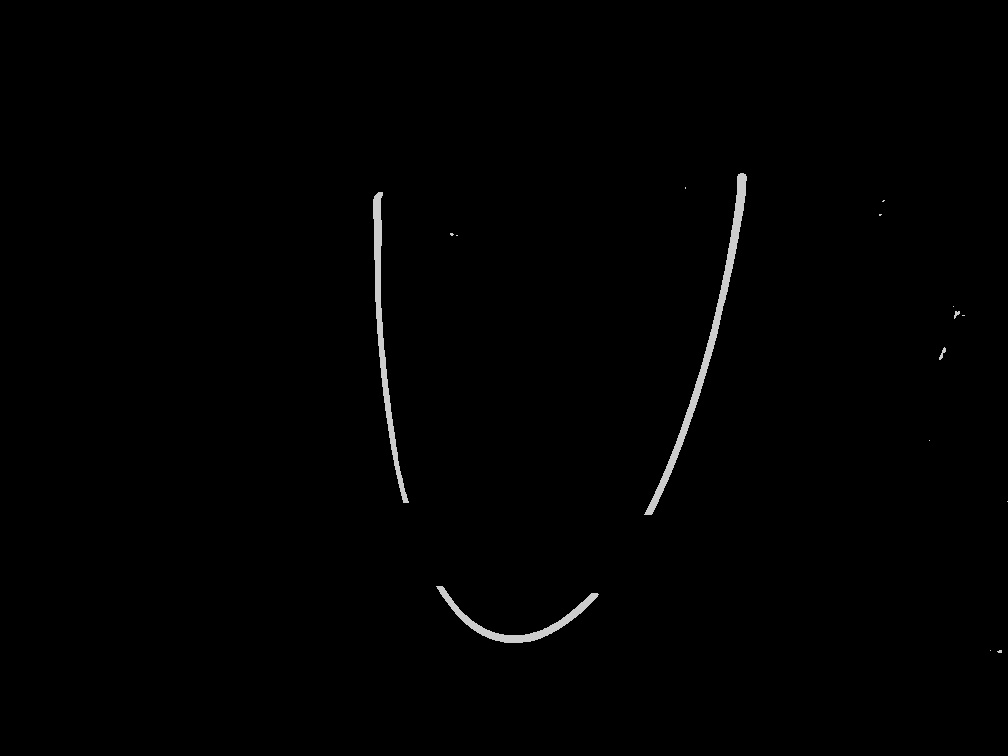
\includegraphics[scale=0.1]{exemplo1WithoutAxis.jpg}}
    \subfigure
        {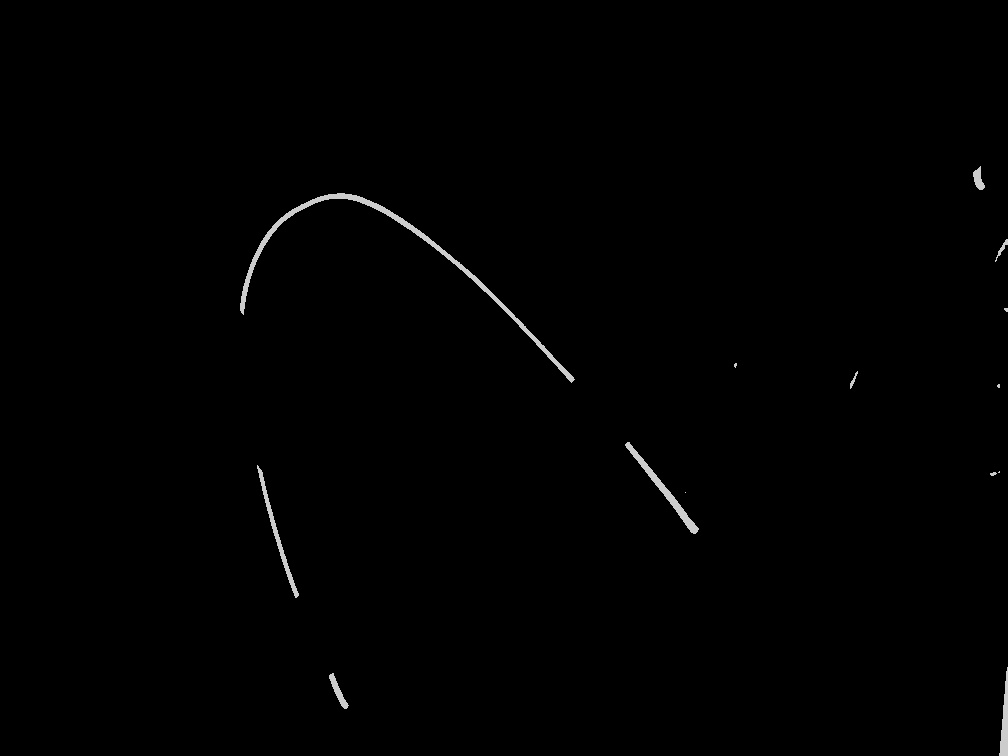
\includegraphics[scale=0.1]{exemplo2WithoutAxis.jpg}}
    \subfigure
        {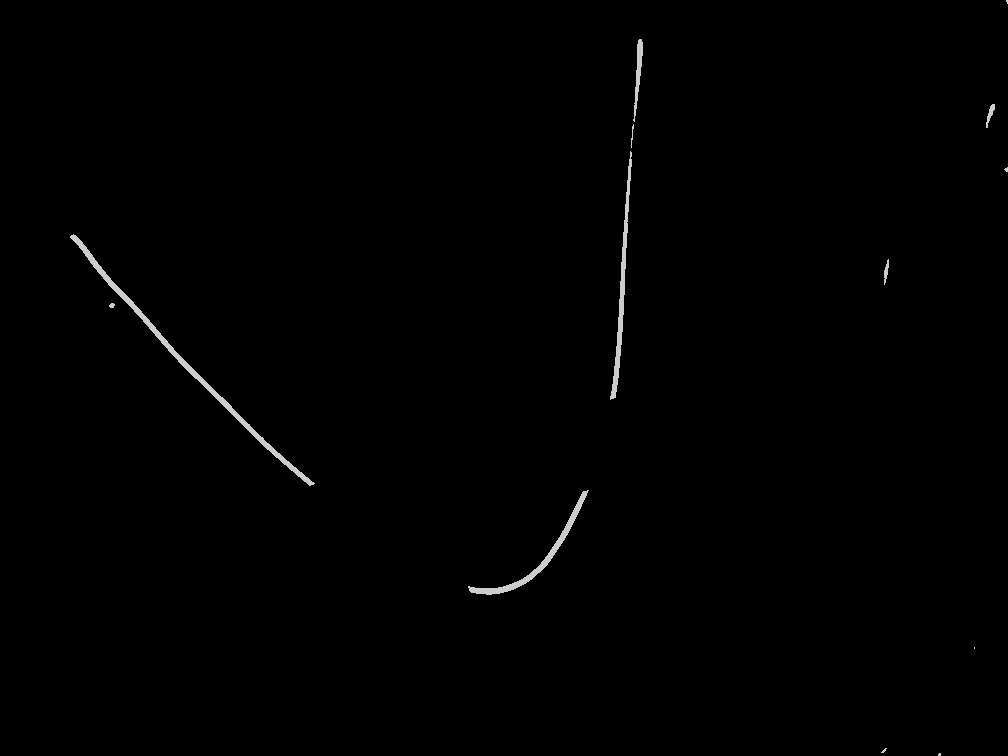
\includegraphics[scale=0.1]{exemplo3WithoutAxis.jpg}}
    \caption{Imagens após remoção dos eixos }
    \end{figure}

\subsection{Identificar a parábola}

    \subsubsection{Identificação dos pontos}
    Foi utilizado Hough para descobrir pequenas linhas que representariam os pontos dentro da parabola.
    \subsubsection{Rotação dos pontos para o eixo \(XY\)}
    Usando a reta do eixo \(X\) como base, pegou o ângulo de inclinação dela, e todos pontos foram rotacionados para o eixo \(XY\), utilizando a matriz de rotação.
    \subsubsection{Cálculo da parábola}
    Utilizando mínimos quadráticos com todos os pontos identificados se descobriu a parábola que passasse por eles e que se encaixasse na formulação \(ax^2 + bx + c = y\).

\subsection{Desenhar a parábola}

Para desenhar a párabola se pegou os pontos de acordo com a equação e rotacionou de volta pela matriz de rotação para o plano do da imagem e desenhou os seus pontos nela.

\begin{figure}[h!]
   \centering
    \subfigure
        {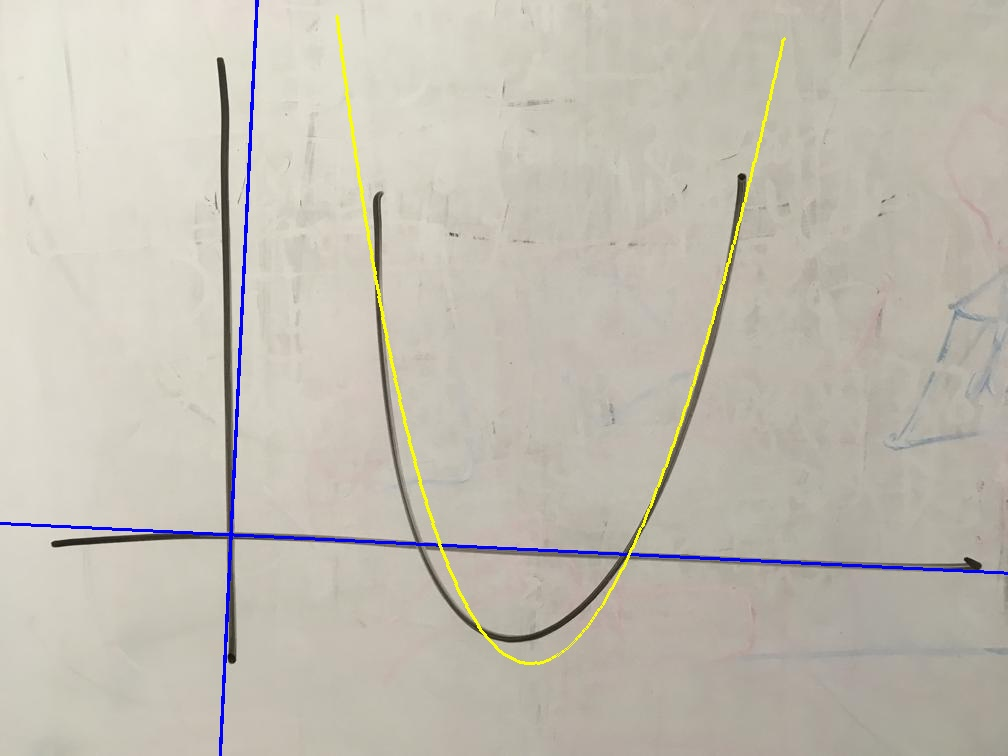
\includegraphics[scale=0.1]{exemplo1ParaboleImage.jpg}}
    \subfigure
        {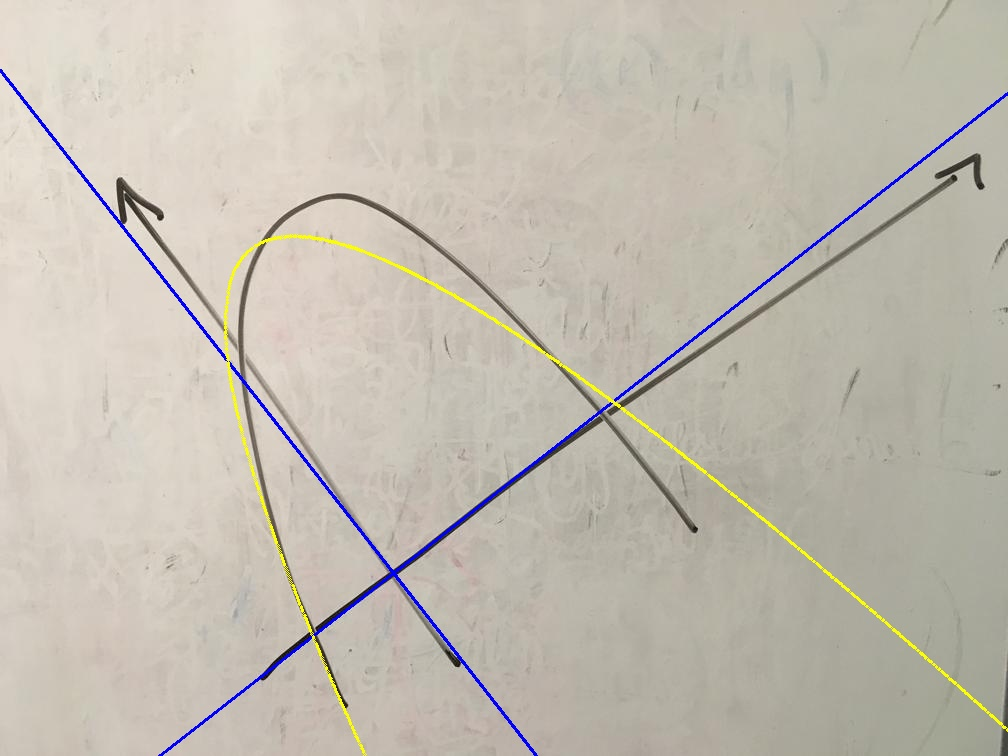
\includegraphics[scale=0.1]{exemplo2ParaboleImage.jpg}}
    \subfigure
        {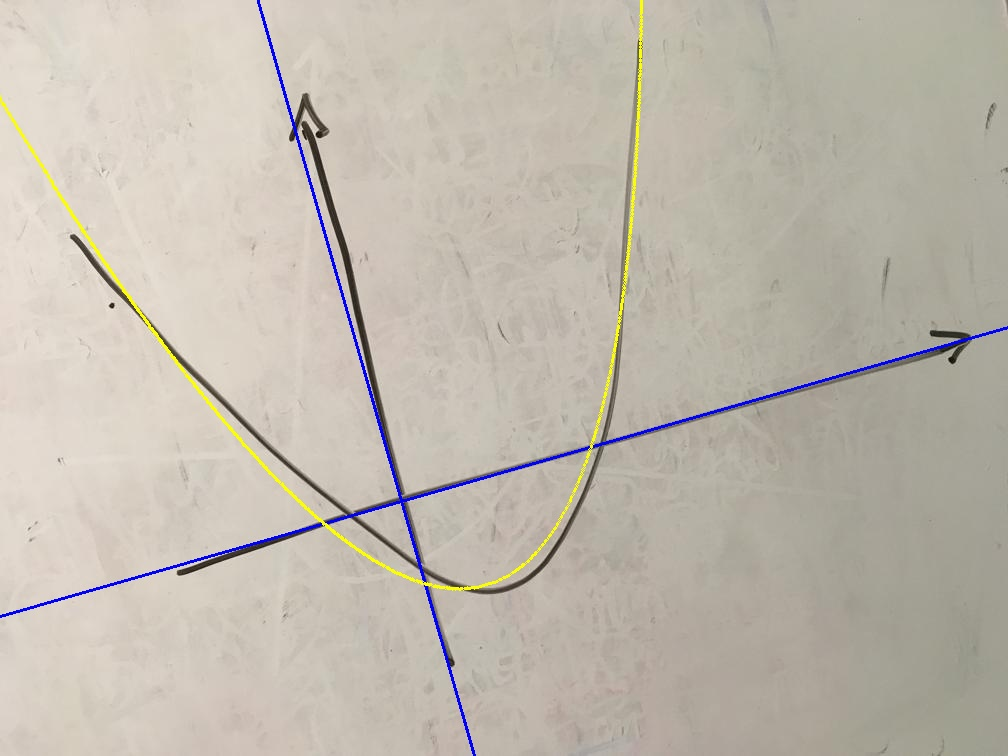
\includegraphics[scale=0.1]{exemplo3ParaboleImage.jpg}}
    \caption{Resultado do trabalho }
\end{figure}
    
    % \[
    % A = 
    %     \begin{bmatrix}
    %     x_1^2   & x_1 & 1 \\
    %     x_2^2   & x_2 & 1 \\
    %     \hdotsfor{3} \\
    %     x_n^2   & x_n & 1 \\
    %     \end{bmatrix}
    % B = 
    %     \begin{bmatrix}
    %     y_1 \\
    %     y_2 \\
    %     \hdotsfor{1} \\
    %     y_n \\
    %     \end{bmatrix}
    % X = 
    %     \begin{bmatrix}
    %     a &  b & c
    %     \end{bmatrix}
    % \]
    
    % \(    A ^ T * A * X = A ^ T * B \)
\end{document}
